%using notation desc for technical names/concepts that should be described in
% our `technical dictionary`. Ref is used as a request for a  regular citation.
\section{Graphical User Interface}

The Graphical User Interface (GUI) is a template- and AJAX-based web
application which uses \django{}'s template system to implement the View part of
the MVC-principle\cite{mvc}.
Each webpage is a template populated through Python code before it is delivered
to the Web server, and ultimately the requesting Web browser.

Additional data that needs to be sent to a Web page, e.g. the user interacts
with the GUI, is requested through JavaScript and AJAX-calls and then gets added to
the already loaded DOM in the web
browser.

\subsection{Structure}

The pages of the GUI are organised in the structure presented in Figure
\ref{fig:gui_structure}, which is very similar to the way BHTB organised its front end.

\begin{figure}[ht!]
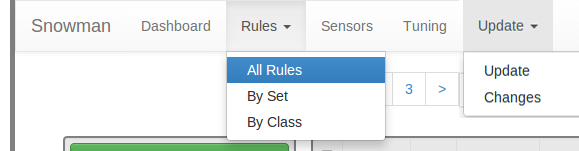
\includegraphics[width=130mm]{./img/gui_menu.png}
\caption{GUI Structure}
\label{fig:gui_structure}
\end{figure}

\subsection{Design}

The GUI is designed with simplicity and minimalism in mind, which is achieved
partially by using Bootstrap that has a lot of default no-nonsense design elements. But we
also opted for using a lot of primary colors and simple lines to
make it aesthetically pleasing.

\subsection{Overview of Central GUI Features}
\subsubsection{Content Prefetching}
One of the main features of our GUI design is our use of prefetching to speed
up loading. Instead of loading absolutely everything into the web browser DOM,
like our predecessor BHTB did, we instead initially only load the first page or
page elements. This is designed to reduce loading times.

We then silently in the background load in any element the user might want to
see next, through AJAX calls. When the user then interacts with the GUI, the
next elements are shown to the user. The next-next elements are also loaded
through AJAX calls so that they are ready. This ensures that the user always has
immediate response from any interaction done with the GUI, while keeping loading times to a bare minimum.


\subsubsection{Rules Page (Figure \ref{fig:gui_rules})}

\begin{figure}[ht!]
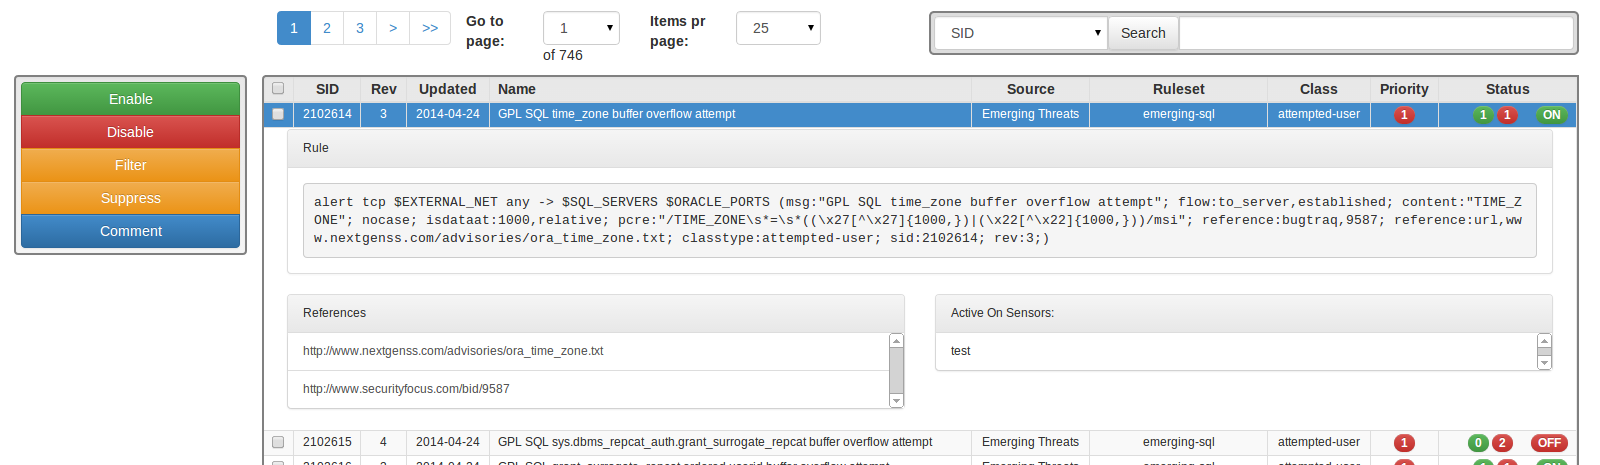
\includegraphics[width=150mm]{./img/gui_rules.png}
\caption{Rules page}
\label{fig:gui_rules}
\end{figure}

This page serves as the complete list of all rules currently residing in the
central database. Because the central database can contain hundreds of
thousands of rules, this list is paginated. Pages are loaded using AJAX calls to
prefetch them as needed. Each row in the list can be clicked on, which expands
an area containing additional information about the rule in question. 

We anticipate that the main use of this page is going to be utilizing the search
function to find a specific rule or rules and then either retrieve information about them
or otherwise manipulate them.

Rules can be tuned by checking the checkbox associated with the rule in question
and then pressing the button that represents the desired function in the box to
the left. 
\newpage
\subsubsection{Rulesets Page (Figure \ref{fig:gui_rulesets})}

\begin{figure}[ht!]
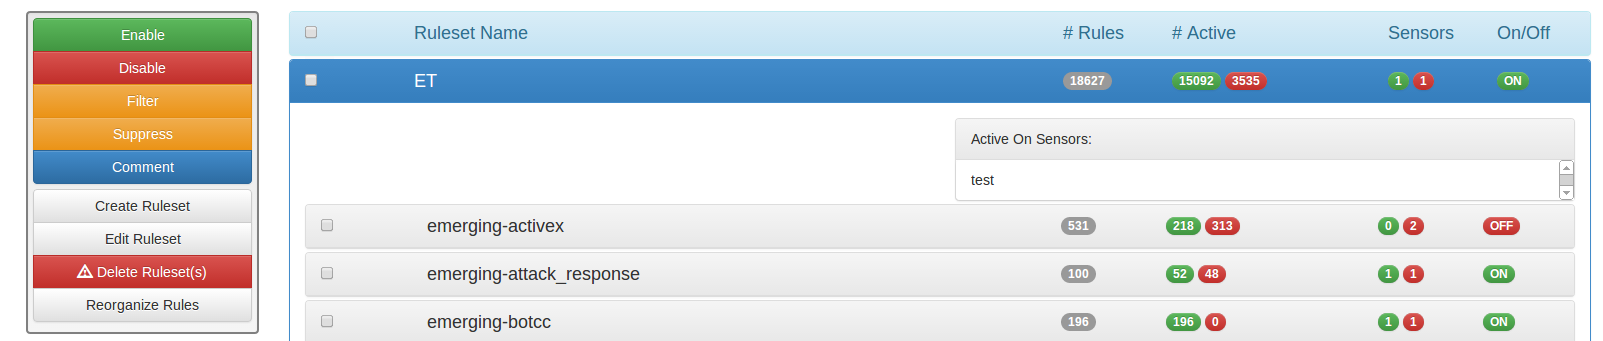
\includegraphics[width=150mm]{./img/gui_rulesets.png}
\caption{Rulesets page}
\label{fig:gui_rulesets}
\end{figure}

The rulesets page consists of a list of all the rulesets stored in the
central database. Each row contains meta information about the ruleset, such as
the number of rules in the ruleset and so on. 

A special feature of the ruleset page is that since Snowman allows the user to
structure rulesets in a hierarchical tree, the ruleset list will initially only
show the tree roots. If the ruleset has child rulesets associated with it, those
will be listed once the user click on the ruleset and opens up the additional
information area. 

The list controls also contain functionality for creating, editing, deleting and
reorganizing the rulesets, as well as the ability to turn them on or off either
globally or on a per sensor basis.

We also have a very similar page for the sensor list, which also allows the user
to arrange sensors in a hierarchical tree. Because it is almost identical, it is not detailed in the report.

\subsubsection{Updates and Changes (Figures \ref{fig:gui_update_progressbar} and
\ref{fig:gui_update_changes})}

One of the big requests from Avdeling BKI when it came to improvements of
features of BHTB was the need to get more feedback from the update process, as
BHTB only told you about the status after it was done, leaving the user without
further information.


\begin{figure}[ht!]
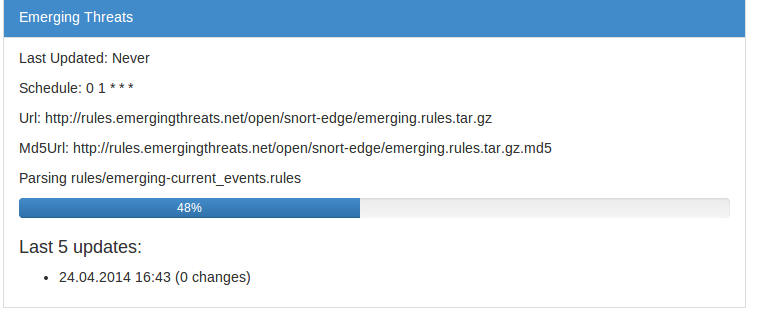
\includegraphics[width=150mm]{./img/gui_update_progressbar.png}
\caption{Update progressbar}
\label{fig:gui_update_progressbar}
\end{figure}

To solve this, we added a continuously updating progressbar which tells the user
what the system is currently doing and give a rough estimate of the percentage
of completion. 

Another requested feature was the ability to see what was changed during an
update. We provide a list for this, which contains each update and its various
changes. 

\begin{figure}[ht!]
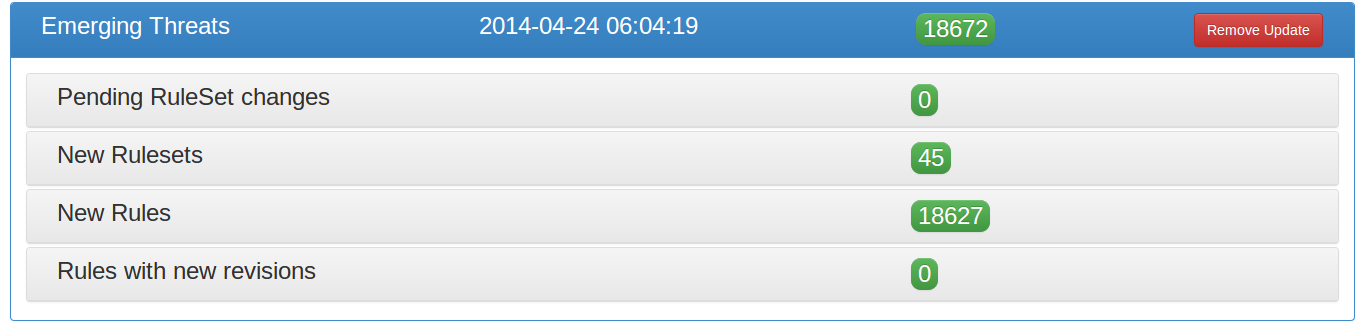
\includegraphics[width=150mm]{./img/gui_update_changes.png}
\caption{Update changes}
\label{fig:gui_update_changes}
\end{figure}

The list details any new rulesets, rules or rule revisions an update
might have brought with it, as well as a list of rules that have been moved from
one ruleset to another. 
Once the user has finished checking out the changes from one update, the user
can remove the update from the list. This makes the list a backlog tool, rather
than a perpetually long list or some sort of time limited list (updates in
the last 7 days or similar). 
This gives the user a good overview of what has changed since the last time the
user checked the list.

\subsubsection{Form Validation and Feedback (Figure
\ref{fig:gui_form_validation})}

One challenge that web frontends always face are forms, as they are a means to
alter data in the database and thus become a security challenge. So when
utilizing forms, it is important to protect the database against both attackers and user errors.

There are three basic steps to implement protection against these
security issues:
\begin{enumerate}
\item Validate the data provided by the form.
\item Make sure the user cannot input something he/she should not.
\item To never let any raw strings or values from the form be directly inserted
into a database query.
\end{enumerate}

The third protection is the most important one as it prevents SQL
injection attacks, which are attacks where SQL code is input into the form, letting the attacker carry out his/her own queries,
leading to total database compromise.
This problem is solved through a technique called prepared statements, which
make sure a query does not do anything it is not supposed to before the query is actually
executed on the database. This protection is implemented in our system through
Django's internal protection mechanisms.

The first and second protection is something we have implemented ourselves in 
both our frontend and our backend. We make sure that the user can never input
invalid values into any form by having Javascript validate the input. So if a user inputs characters
where only numbers are allowed, the user will be notified immediately and not
allowed to submit the form until it is corrected. And this is done before
anything is ever sent from the browser to the server.

But if the user has input all valid values, we still validate all the data at
the backend before we store anything in the database. This means verifying
that any referenced object ID actually exists and making sure the provided IP
address is actually valid (within the 0.0.0.0/0 - 255.255.255.255/32 range). If
anything is out of place, a message is sent back to the user about it.

\begin{figure}[ht!]
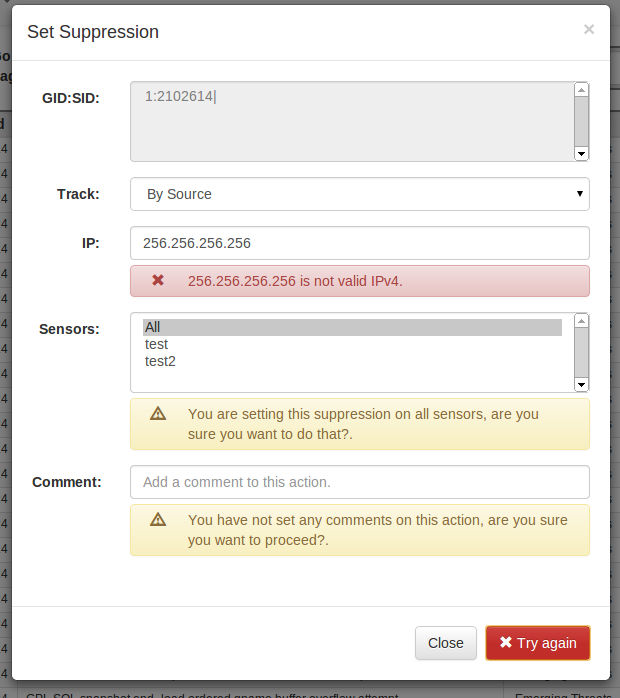
\includegraphics[width=150mm]{./img/gui_form_validation.png}
\caption{Form validation}
\label{fig:gui_form_validation}
\end{figure}


